%!TEX root = documento.tex

%% Preâmbulo (configurações, pacotes e tudo mais)

%% Preambulo LaTeX: Define classes e características do documento
%% Definição do docuemnto
\documentclass[
	%article,			% Define que este será um artigo (e não uma tese/monografia/relatório)
	12pt,				% Fonte: 12pt
	oneside,			% Impressão: oneside = 1 face, twoside = 2 faces (frente-e-verso)
    %openright,			% capítulos começam em página ímpar (use apenas se usar "twoside")
	a4paper,			% Tamanho do Papel: A4
    chapter=TITLE,		% Todos os capítulos devem ficam em caixa alta
    section=TITLE,		% Todas as seções devem ficar em caixa alta
	english,			% Adiciona Idioma para Hifenização: Inglês
    %spanish,			% Adiciona Idioma para Hifenização: Espanhol
    %french,			% Adiciona Idioma para Hifenização: Francês
	brazil				% Adiciona Idioma para Hifenização: Português do Brasil (o último idioma se torna o principal do documento)
]{abntex2}				% Utilizar ABNTeX2





%% Tipografia
%% Abra este arquivo e selecione uma das opções de fonte nele. A padrão é Times.
%% Tipografia / Fontes
%% AVISO: Todas essas fontes são *bastante semelhantes* aos nomes com as quais as descrevo. Entenda: são iguais, só que oficialmente com outro nome.

%% %%%%%%%%%%%%%%%%%%%%%%%%%%%%%%%%%%%%%%%%%%%%%%%%%%%%% %%
%% Comente todas as outras fontes que você não vai usar! %%
%% %%%%%%%%%%%%%%%%%%%%%%%%%%%%%%%%%%%%%%%%%%%%%%%%%%%%% %%

%% Latin Modern (fonte padrão do LaTeX, Computer Modern, mas com suporte a caracteres acentuados)
%% Considerada a mais clássica e bonita
%\usepackage{lmodern}



%% Times
%% Considerada a mais confortável de ler quando impresso
%%\usepackage{mathptmx}

%% Variação da mesma fonte, com minúsculas diferenças entre uma e outra (coisas bastante técnicas como kerning, aliasing e afins) - Essa tem revisões frequentes
%\usepackage{newtxtext} \usepackage{newtxmath}



%% Arial
%% Considerada mais confortável de ler num computador
%% ** Oficialmente recomendada pelo manual de formatação do IFPI **
\usepackage{helvet} \renewcommand{\familydefault}{\sfdefault}



%% Palatino
%% Uma opção mais elegante à Times
%\usepackage{newpxtext}



%% Kepler
%% Variação evoluída da Palatino, com várias pequenas diferenças e refinamentos
%\usepackage{kpfonts}



%% Libertine
%% Uma fonte estilo Serif comum no Linux
%\usepackage{libertine} %\usepackage[libertine]{newtxmath}



%% Pacotes usados pelo documento (se não entender não mexa, hehehe)
\usepackage{courier}                    % Permite a utilização da fonte Courier (para códigos-fonte)
\usepackage[T1]{fontenc}				% Seleção de códigos de fonte.
\usepackage[utf8]{inputenc}				% Codificação do documento (conversão automática dos acentos)
\usepackage{indentfirst}				% Indenta o primeiro parágrafo de cada seção.
\usepackage{nomencl} 					% Usado pela Lista de símbolos
\usepackage{color}						% Controle das cores
\usepackage{graphicx}					% Inclusão de gráficos
\usepackage{float}						% Melhorias para posicionamento de gráficos e tabelas
\usepackage{microtype} 					% Melhorias na justificação
\usepackage{lastpage}   		        % Dá acesso ao número da última página do documento
\usepackage{booktabs}					% Comandos para tabelas
\usepackage{multirow, array}			% Múltiplas linhas e colunas em tabelas
\usepackage{titlesec}                   % Permite criar múltiplas sub seções
\usepackage[table,xcdraw]{xcolor}       % Cores para algumas tabelas especiais
% \usepackage[brazilian,hyperpageref]{backref}	 % Inclui nas Referências as páginas onde há as citações
\usepackage{simplecd}                   % Pacote para gerar capa do CD
\usepackage[final]{pdfpages}            % Pacote para incluir um PDF dentro de outro (ficha catalográfica)
\usepackage{csquotes}



%% Adiciona as alterações do ABNTeX-IFPI
\usepackage{abntex-ifpi/abntex-ifpi}

% Modificações do ABNTeX para o IFPI
\usepackage{abntex-ifpi/tikz-uml}	    % Pacote Tikz UML para criar UML no LaTeX





%% Metadados
%% Configurações dos metadados do PDF
\makeatletter
\hypersetup{
  pdftitle={\@title}, 
  pdfauthor={\@author},
  pdfsubject={\@title},
  pdfcreator={LaTeX, abntex2, {abnTeX\-ifpi}},
  %% Coloque aqui suas palavras-chave, cada uma entre chaves: {palavra}{palavra}{outra palavra}...
  pdfkeywords={palavra 1}{palavra 2}{palavra 3}{palavra 4}{palavra 5},
  colorlinks=true,			% Visual dos Links: false = caixas; true = colorido
  linkcolor=cor-link,		% Cor dos Links Internos (preto)
  citecolor=cor-link,		% Cor de Links para Bibliografia (preto)
  filecolor=cor-link,		% Cor para Links a Arquivos (preto)
  urlcolor=cor-link,		% Cor para Links a URLs (preto)
  bookmarksdepth=4
}
\makeatother



%% Metadados
%% %%%%%%%%%%%%%%%%%%%%%%%%%%%%%%%%%%%%%%%%%%%%%%%% %%
%% Metadados do trabalho
%% AVISO: Todos esses dados serão automaticamente convertidos para caixa alta onde necessário
%% %%%%%%%%%%%%%%%%%%%%%%%%%%%%%%%%%%%%%%%%%%%%%%%% %%

%% Título
\titulo{Registro de Ponto Digital}

%% Autor
\autor{Karielly de Carvalho}

%% Nome do Curso (usado para a Capa do CD)
\nomedocurso{Análise e Desenvolvimento de Sistemas}

%% Local de publicação
\local{Picos, Piauí}

%% Preâmbulo do trabalho
\preambulo{Trabalho de Conclusão de Curso (Relatório Técnico de Software) apresentado como exigência parcial para obtenção do diploma do Curso de Análise e Desenvolvimento de Sistemas do Instituto Federal de Educação, Ciência e Tecnologia do Piauí, Campus Picos.}

%% Orientador
%% "M\textsuperscript{e}." = Abreviação oficial para "Mestre"
\orientador{Prof. M\textsuperscript{e}. Jesiel Viana da Silva}

%% Tipo de Trabalho
%% - Monografia
%% - Tese (Mestrado)
%% - Tese (Doutorado)
%% - Relatório técnico
\tipotrabalho{Relatório Técnico de Software}

%% Data do Trabalho
\data{2025}

%% Nome da Instituição (para a capa)
\instituicao{INSTITUTO FEDERAL DE EDUCAÇÃO, CIÊNCIA E TECNOLOGIA DO PIAUÍ
\\
CAMPUS PICOS
\\
TECNOLOGIA EM ANÁLISE E DESENVOLVIMENTO DE SISTEMAS}

%% Primeiro membro da banca examinadora
\membroum{Prof. M\textsuperscript{e}. Aislan Rafael Rodrigues de Sousa}

%% Segundo membro da banca examinadora
\membrodois{Prof. M\textsuperscript{e}. 
João Paulo Lima do Nascimento}

%% Terceiro membro da banca examinadora
%\membrotres{Prof. Dr. Xxxxxx Xxxxx}

%% Data da apresentação do trabalho
%% Se não souber a data da apresentação, utilize \underline{\hspace{3.5cm}}
%% Isso cria um sublinhado de 3.5cm, onde você pode escrever a data depois!
%\dataapresentacao{02 de Outubro de 2023}
\dataapresentacao{\underline{\hspace{1.0cm}}/\underline{\hspace{1.0cm}}/\underline{\hspace{1.75cm}}}



%% Configuração do "Citado nas páginas"
%% Configuração das Citações

%% Estilo
%\usepackage[num]{abntex2cite}			% Citações numéricas
% \usepackage[abnt-nbr10520=1988, alf, 
% abnt-emphasize = bf, 
% abnt-etal-list = 3,
% abnt-etal-text = it, 
% abnt-and-type = &, 
% abnt-last-names = abnt, 
% abnt-repeated-author-omit = no]{abntex2cite}			% Citações "AUTOR, ano"


% Definição do negrito

%% Colocar entre parênteses ou colchetes?
%% Padrão: Parênteses
%% * Fica mais agradável usar colchetes quando se usa citações numéricas
%\citebrackets[]							% Comente essa linha e o documento usará parênteses


%% Configura o "Citado nas Páginas ..." nas referências
%% Não mexa nesse:
% \renewcommand{\backref}{}

%% Esse é o texto do "Citado nas páginas ..."
% \renewcommand*{\backrefalt}[4]{
% 	\ifcase #1
% 		Nenhuma citação no texto.
% 	\or
% 		Citado na página #2.
% 	\else
% 		Citado #1 vezes nas páginas #2.
% 	\fi}

% ----------------------------------------------------------
% Referências e Citações no padrão da ABNT 2023
% ----------------------------------------------------------

\usepackage[style=abnt,
    backend=biber,
    maxbibnames=99,
    mincitenames=1,
    maxcitenames=3,
    backref=true,
    hyperref=true,
    giveninits=false,
    uniquename=false,
    uniquelist=false]{biblatex}

% Modificar a formatação do título do artigo para negrito
% \DeclareFieldFormat[article]{title}{\mkbibbold{#1}}

% Modificar a formatação do sobrenome em minúsculas
\renewcommand*{\mkbibnamefamily}[1]{#1}%

\addbibresource{bibliografia.bib}



%% Cores
%% Cores do Documento

%% Cor dos Links do PDF
%% Usando preta você "esconde" os links
\definecolor{cor-link}{RGB}{0,0,0}

%% Usando azul os links ficam visíveis (ruim para impressão)
%\definecolor{cor-link}{RGB}{8,40,75}



%% Cor para os quadros
%% Dê preferência a cores escuras.
%% Boa referência para cores: https://material.io/guidelines/style/color.html#color-color-palette
\definecolor{cor-quadro}{RGB}{5,28,63}		% Azul Escuro



%% Espaçamentos
%% Espaçamentos
%% O tamanho do parágrafo é dado por:
\setlength{\parindent}{1.5cm}

%% Espaçamento entre um parágrafo e outro:
%% O abntex diz: "tente também \onelineskip"
\setlength{\parskip}{0cm}


%% Início do Documento
\begin{document}

%% Documento será escrito em Português do Brasil
\selectlanguage{brazil}

%% Elementos pré-textuais: capa, folha de rosto, dedicatória, listas, sumário, etc.
%% %%%%%%%%%%%%%%%%%%%%%%%%%%%%%%%%%%%%%%%%% %%
%% Elementos Pré Textuais
%% ----------------------
%% 
%% Segundo o manual do IFPI, eles devem ser os seguintes (nessa ordem):
%%  1. Capa (obrigatório)
%%  2. Folha de rosto (obrigatório)
%%  3. Errata (opcional)
%%  4. Folha de aprovação (obrigatório)
%%  5. Dedicatória (opcional)
%%  6. Agradecimentos (opcional)
%%  7. Epígrafe (opcional)
%%  8. Resumo (obrigatório)
%%  9. Abstract/Resumo em outra língua (obrigatório)
%% 10. Lista de Ilustrações (opcional)
%% 11. Lista de Tabelas (opcional)
%% 12. Lista de Abreviaturas e Siglas (opcional)
%% 13. Lista de Símbolos (opcional)
%% 14. Sumário (obrigatório)
%% %%%%%%%%%%%%%%%%%%%%%%%%%%%%%%%%%%%%%%%%% %%

%% 01: Capa
\imprimircapa



%% 02: Folha de Rosto
%% OBS: O asterisco indica que haverá ficha bibliográfica (só funciona para impressão frente-e-verso)
\imprimirfolhaderosto*



%% Ficha Catalográfica (acho que é melhor adicionar via \includepdf depois)
%%% Ficha Catalográfica
%%
%% Este template cria um quadro semelhante a ficha catalográfica oficial.
%% É melhor usar \includepdf depois que a ficha oficial estiver em mãos.

%% Caso tenha o arquivo PDF da ficha
%% A ficha catalográfica do IFPI pode ser gerada através neste link: https://sistemas.ifpi.edu.br/fichacatalografica/
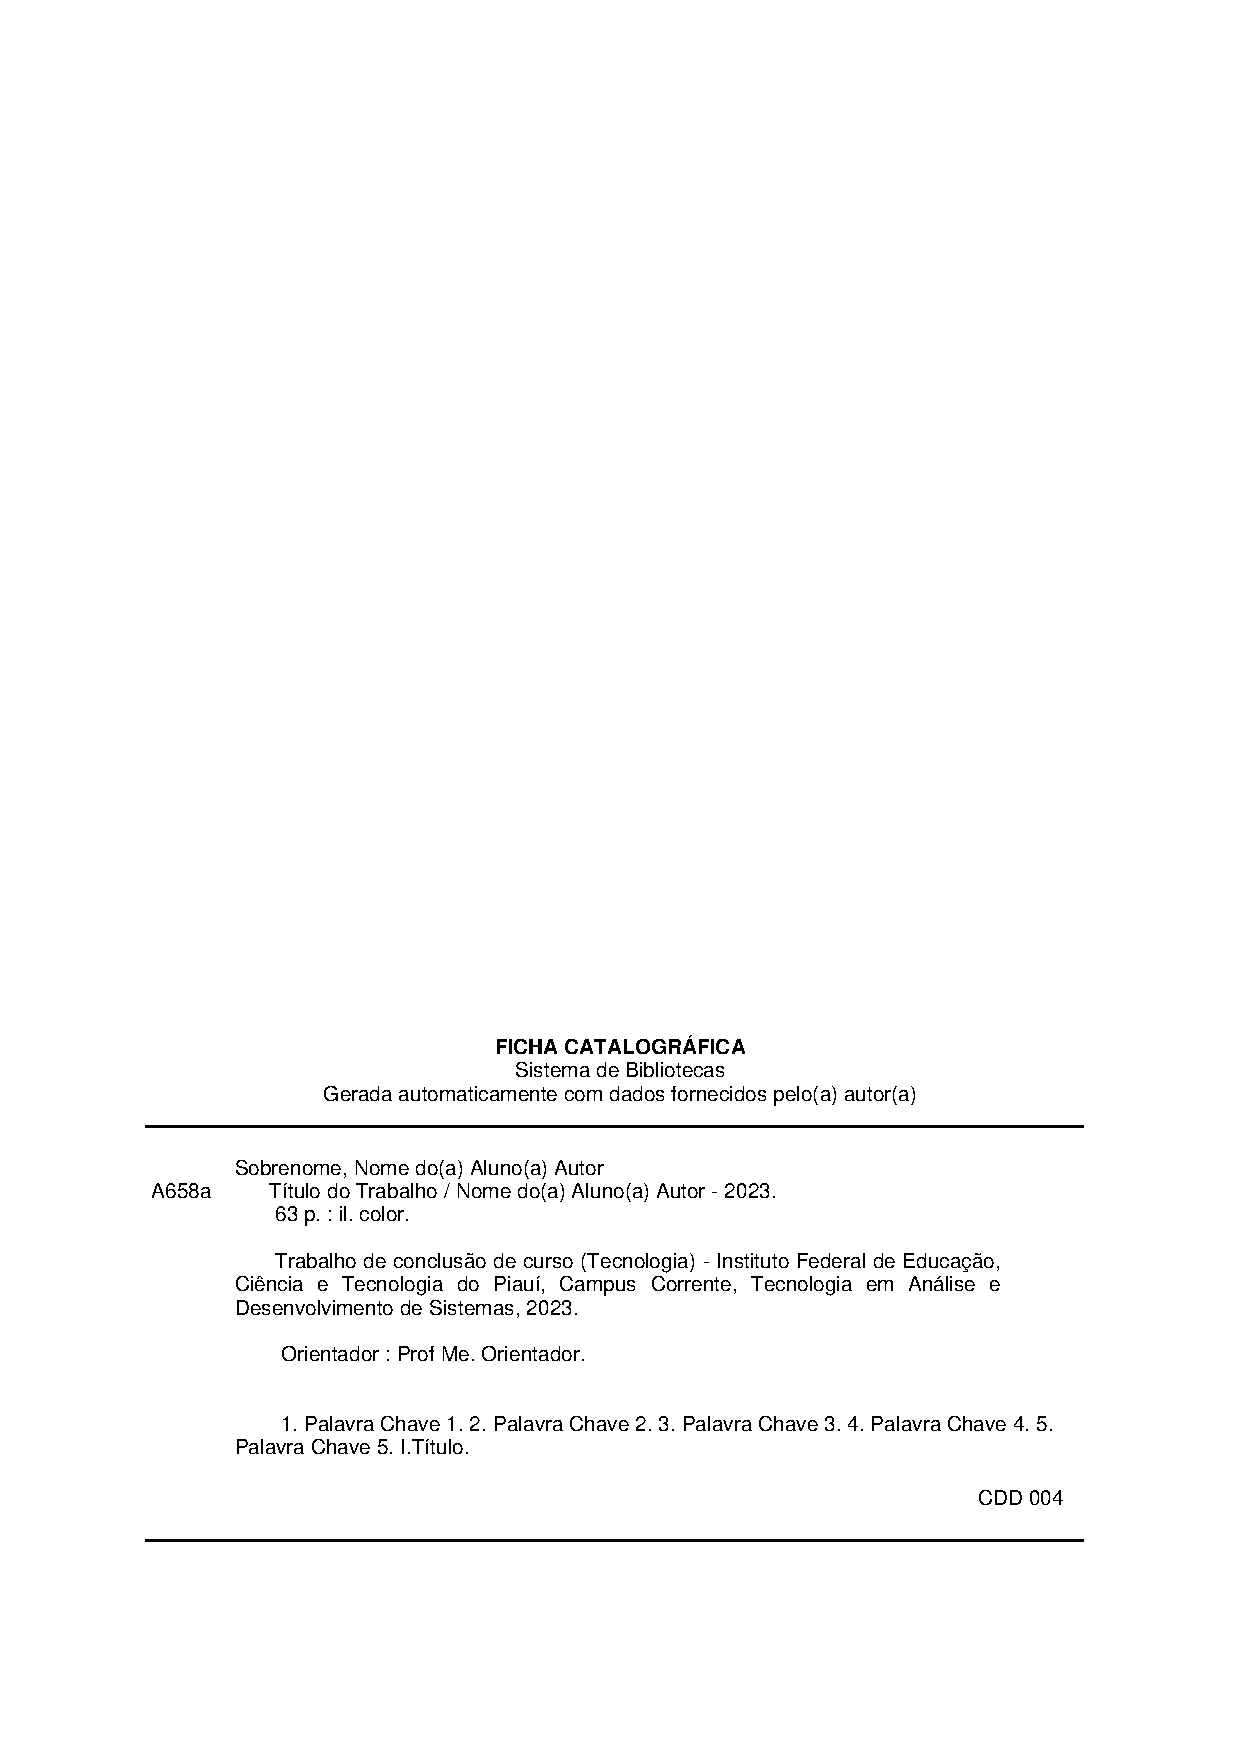
\includepdf{pre-textual/ficha-catalografica.pdf}

%% Caso queira fazer a ficha "tradicional" (este serve apenas como um modelo)
%\begin{fichacatalografica}
%	\sffamily
%	\vspace*{\fill}					% Posição vertical
%	\begin{center}					% Minipage Centralizado
%	\fbox{\begin{minipage}[c][8cm]{13.5cm}		% Largura
%	\small
%	\imprimirautor
%	
%	\hspace{0.5cm} \imprimirtitulo  / \imprimirautor. --
%	\imprimirlocal, \imprimirdata-
%	
%	\hspace{0.5cm} \thelastpage p. : il. (algumas color.) ; 30 cm.\\
%	
%	\hspace{0.5cm} \imprimirorientadorRotulo~\imprimirorientador\\
%	
%	\hspace{0.5cm}
%	\parbox[t]{\textwidth}{\imprimirtipotrabalho~--~\imprimirinstituicao,
%	\imprimirdata.}\\
%	
%	\hspace{0.5cm}
%		1. Palavra-chave1.
%		2. Palavra-chave2.
%		2. Palavra-chave3.
%		I. Orientador.
%		II. Universidade xxx.
%		III. Faculdade de xxx.
%		IV. Título 			
%	\end{minipage}}
%	\end{center}
%\end{fichacatalografica}


%% 03: Errata
%% Errata
%\begin{errata}
%Elemento opcional da norma ABNT NBR14724 de 2011. Exemplo:
%
%\vspace{\onelineskip}
%
%FERRIGNO, C. R. A. \textbf{Tratamento de neoplasias ósseas apendiculares com reimplantação de enxerto ósseo autólogo autoclavado associado ao plasma rico em plaquetas}: estudo crítico na cirurgia de preservação de membro em cães. 2011. 128 f. Tese (Livre-Docência) - Faculdade de Medicina Veterinária e Zootecnia, Universidade de São Paulo, São Paulo, 2011.

%% Tabela de exemplo com os erros
%\begin{table}[htb]
%\center
%\footnotesize
%\begin{tabular}{|p{1.4cm}|p{1cm}|p{3cm}|p{3cm}|}
%  \hline
%   \textbf{Folha} & \textbf{Linha}  & \textbf{Onde se lê}  & \textbf{Leia-se}  \\
%    \hline
%    1 & 10 & auto-conclavo & autoconclavo\\
%   \hline
%\end{tabular}
%\end{table}
%
%\end{errata}



%% 04: Folha de Aprovação
\imprimirfolhadeaprovacao
%% Use esta se forem 4 membros na banca:
%\imprimirfolhadeaprovacaoduascolunas



%% 05: Dedicatória
%% Dedicatória do seu trabalho
\begin{dedicatoria}
	%% Empura o texto a seguir para a parte de baixo da página
	\vspace*{\fill}
    
    %% Alinhado a Direita
    \center
    \begin{flushright}
    	Dedico este trabalho à minha família, cujo apoio e incentivo tornaram possível esta nova jornada.
    \end{flushright}
    
    %% Descomente a linha seguir para deixar o texto centralizado verticalmente na página
    %% Lembre de comentar o "\begin{}" e "\end{}" acima para centralizar o texto da dedicatória.
	%\vspace*{\fill}
\end{dedicatoria}



%% 06: Agradecimentos
\chapter*{Agradecimentos}

Agradeço primeiramente a Deus, por me conceder sabedoria, saúde e força durante toda esta jornada acadêmica.

Ao meu orientador, professor Aislan Rafael, pela dedicação, paciência e ótimas orientações ao longo do desenvolvimento deste trabalho.

À minha família, especialmente aos meus pais, Juvan Luís de Carvalho e Alessandra Rodrigues de Carvalho, por todo amor, apoio incondicional e incentivo desde o início da minha trajetória — sem vocês, nada disso seria possível. À minha irmã, Fernanda Monique de Carvalho, e ao meu irmão, Levi Rodrigues de Carvalho, pelo companheirismo e carinho. À minha sobrinha, Aurora Monique de Carvalho, que, com sua doçura e alegria, iluminou muitos dos meus dias e me deu ainda mais motivação para seguir em frente.

Ao meu namorado, Jean Carlos Rodrigues Sousa, por todo incentivo e parceria nos momentos mais desafiadores desta caminhada. Sua presença foi importante para que eu chegasse até aqui, e sua confiança em mim fez toda a diferença.

A todos que, de alguma forma, contribuíram para a realização deste trabalho, deixo o meu mais sincero agradecimento.




%% 07: Epígrafe
%% Epígrafe
%% Uma frase que lhe inspira ou a qual lhe inspirou a fazer este trabalho
\begin{epigrafe}
\vspace*{\fill}
\begin{flushright}
\emph{"A tecnologia move o mundo."} \\
\vspace{0.5cm}
— Steve Jobs
\end{flushright}
\end{epigrafe}




%% 08: Resumo
% %% Resumo
% \begin{resumo}
% Apresentação concisa dos pontos relevantes do documento. Deve Informar ao leitor 
% finalidades, metodologia, resultados e conclusões do documento, de tal forma que 
% este possa, inclusive, dispensar a consulta ao original. Deve-se usar o verbo na voz 
% ativa e na terceira pessoa do singular, contendo de 150 a 500 palavras. O resumo 
% deve ser composto de uma sequência de frases concisas, afirmativas e não de 
% enumeração de tópicos. Recomenda-se o uso de parágrafo único, mesma fonte do 
% trabalho, e espaçamento entrelinhas 1,5. Resumo resumo resumo resumo resumo 
% resumo resumo resumo resumo resumo resumo resumo resumo resumo resumo 
% resumo resumo resumo resumo resumo resumo resumo resumo resumo resumo 
% resumo resumo resumo resumo resumo resumo resumo resumo resumo resumo 
% resumo ( ASSOCIAÇÃO BRASILEIRA DE NORMAS TÉCNICAS, 2021).
% \vspace{\onelineskip}
% \noindent

% \textbf{Palavras-chaves}: Palavra 1; Palavra 2; 
% Palavra 3.
% \end{resumo}

%% 09: Abstract/Resumo em língua estrangeira
%% Abstract (configurado para língua inglesa)
% \begin{resumo}[Abstract]			% Título do Resumo (Abstract = Resumo em inglês)
% \begin{otherlanguage*}{english}		% Língua do texto
% Elemento obrigatório, com as mesmas características do resumo em língua 
% vernácula, digitado em folha separada (em inglês Abstract, em espanhol Resumen, 
% em francês Résumé, por exemplo). Abstract abstract abstract abstract abstract 
% abstract abstract abstract abstract abstract abstract abstract abstract abstract 
% abstract abstract abstract abstract abstract abstract abstract abstract abstract 
% abstract abstract abstract abstract abstract abstract abstract abstract abstract 
% abstract abstract abstract. ( ASSOCIAÇÃO BRASILEIRA DE NORMAS TÉCNICAS, 2021). 

% \vspace{\onelineskip}
% \noindent
% \textbf{Keywords}: Word 1; Word 2; Word 3.
% \end{otherlanguage*}
% \end{resumo}

%% Exemplo de resumo em francês
%\begin{resumo}[Résumé]
% \begin{otherlanguage*}{french}
%    Il s'agit d'un résumé en français.
% 
%   \textbf{Mots-clés}: latex. abntex. publication de textes.
% \end{otherlanguage*}
%\end{resumo}

%% Exemplo de resumo em Espanhol
%\begin{resumo}[Resumen]
% \begin{otherlanguage*}{spanish}
%   Este es el resumen en español.
%  
%   \textbf{Palabras clave}: latex. abntex. publicación de textos.
% \end{otherlanguage*}
%\end{resumo}
% ---



%% 10: Lista de Ilustrações
% %% Lista de Ilustrações
% \pdfbookmark[0]{\listfigurename}{lof}
% \listoffigures*
% \cleardoublepage



%% 11: Lista de Tabelas
% Lista de Tabelas
\pdfbookmark[0]{\listtablename}{lot}
\listoftables*
\cleardoublepage



%% 12: Lista de Abreviaturas e Siglas
%% Lista de Siglas
\begin{siglas}
  \item[ABNT] Associação Brasileira de Normas Técnicas
  \item[CLT] Consolidação das Leis do Trabalho
  \item[CSS] Cascading Style Sheets (Folhas de Estilo em Cascata)
  \item[IFPI] Instituto Federal de Educação, Ciência e Tecnologia do Piauí
  \item[MPE] Micro e Pequenas Empresas
  \item[ORM] Mapeador Objeto-Relacional
  \item[SSR] Server-Side Rendering (Renderização no Lado do Servidor)
  \item[API] Interface de Programação de Aplicação
\end{siglas}




%% 13: Lista de Símbolos
% %% Lista de Símbolos
% %% (esta é apenas uma lista de exemplo)
% \begin{simbolos}
%   \item [\% ] Porcentagem
%   \item [ © ] Copyright
%   \item [ ® ] Marca registrada
%   \item [ \$ ] Dólar
%   \item [ § ] Seção
%   \item[$ \Gamma $] Letra grega Gama
%   \item[$ \Lambda $] Lambda
%   \item[$ \zeta $] Letra grega minúscula zeta
%   \item[$ \in $] Pertence
% \end{simbolos}



%% 14: Sumário (o asterisco retira o próprio sumário do sumário)
\pdfbookmark[0]{\contentsname}{toc}
\tableofcontents*
\cleardoublepage



%% Indica que a partir daqui ficarão os elementos textuais (TCC em si)
\textual

%% Inclui os capítulos do TCC (parte textual)
%% %%%%%%%%%%%%%%%%%%%%%%%%%%%%%%%%%%% %%
%% Elementos Textuais (Capítulos)      %%
%% %%%%%%%%%%%%%%%%%%%%%%%%%%%%%%%%%%% %%
\pagestyle{empty} % Remover cabeçalho com titulo dos capítulos


%% Inclua aqui os capítulos que farão parte do TCC
% ----------------------------------------------------------
% Introdução
% ----------------------------------------------------------
\chapter{Introdução}

A gestão da jornada de trabalho é um elemento crucial para o bom funcionamento das organizações, pois influencia diretamente tanto a conformidade com a legislação quanto a eficiência operacional. No Brasil, o artigo 74 da Consolidação das Leis do Trabalho (CLT)\footnote{\url{https://www.planalto.gov.br/ccivil_03/decreto-lei/del5452.htm}} determina que empresas com mais de 20 colaboradores devem manter o registro de ponto de seus funcionários \cite{brasil1943}. No entanto, micro e pequenas empresas (MPEs) enfrentam desafios significativos nesse aspecto, especialmente devido ao alto custo de sistemas eletrônicos de controle de ponto. Como alternativa, muitas recorrem a métodos manuais, considerados mais acessíveis inicialmente, mas que acabam aumentando os riscos de imprecisões, perdas de dados e até fraudes no acompanhamento das horas trabalhadas, comprometendo a eficácia na gestão do tempo \cite{miranda2023}.
A adoção de sistemas digitais de registro de ponto oferece benefícios importantes. Essas soluções eliminam a necessidade de equipamentos físicos específicos, permitindo o uso de dispositivos já disponíveis, como tablets, smartphones ou computadores. Dessa forma, tornam-se opções mais práticas e econômicas para a gestão eficiente do banco de horas \cite{FlorindoBianchi2022}.
 
De acordo com \textcite{gomes2023}, o registro de ponto digital tem se consolidado como uma solução eficaz para empresas que buscam otimizar a gestão de suas equipes sem comprometer o orçamento. Esse modelo proporciona maior precisão e transparência no acompanhamento das horas trabalhadas, além de reduzir os custos operacionais. Em contrapartida, a permanência no uso de métodos manuais pode levar a falhas significativas na supervisão da jornada de trabalho, prejudicando tanto empregadores quanto empregados. Um monitoramento inadequado impacta negativamente o cumprimento das obrigações legais e a transparência necessária para garantir a confiança mútua entre as partes \cite{abreu2016sistema}.

Este projeto tem como objetivo e desenvolver uma solução digital acessível e eficiente. Para isso, será desenvolvido um sistema de registro de ponto digital que utiliza tecnologias como escaneamento de QR Code e geolocalização. Essa abordagem busca otimizar o controle das horas trabalhadas, proporcionando maior precisão, autonomia aos funcionários e conformidade com as exigências legais, além de reduzir custos e riscos associados aos métodos manuais. 

Segundo \textcite{gomes2023}, a adoção de sistemas digitais para o registro de ponto oferece uma alternativa prática e econômica para empresas com recursos limitados, enquanto \textcite{mariotti2011} enfatizam que esses sistemas desempenham um papel essencial na melhoria dos processos internos e no cumprimento das normas trabalhistas. Assim, os sistemas digitais não apenas aumentam a eficiência, mas também promovem a transparência e a segurança jurídica para empregadores e funcionários.

\section{Justificativa}
Este projeto visa aprimorar o gerenciamento e controle das horas trabalhadas, beneficiando tanto empresas quanto funcionários, ao modernizar e tornar mais seguro o processo de gestão de pessoas por meio de soluções tecnológicas. Muitas micro e pequenas empresas (MPEs) ainda enfrentam dificuldades para substituir registros manuais por sistemas digitais. Métodos tradicionais, como planilhas e livros de ponto, são suscetíveis a erros humanos e não garantem a segurança necessária, podendo resultar em inconsistências no controle de jornada e problemas trabalhistas \cite{FlorindoBianchi2022}. 

Diante desse cenário, este estudo se torna importante para analisar e desenvolver uma solução digital acessível, segura e eficiente. Além de atender às exigências legais, um sistema digital pode reduzir custos operacionais, otimizar o controle de jornada e fortalecer a transparência nas relações de trabalho. Com isso, há potencial para impactos positivos significativos, como aumento da produtividade, redução de erros manuais e maior satisfação dos colaboradores \cite{gomes2023}.

De acordo com \textcite{Longo2019}, a transformação digital tem impulsionado mudanças rápidas e contínuas nas organizações, reformulando produtos, serviços e processos internos. Essas mudanças afetam diretamente as relações de trabalho e tornam indispensável a adoção de soluções inovadoras para acompanhar a evolução do mercado. Assim, este estudo se justifica pela necessidade de desenvolver uma ferramenta digital que atenda a essas novas demandas, promovendo benefícios para empregadores e funcionários, além de contribuir para a modernização e eficiência da gestão empresarial.


\section{Objetivos}

\subsection{Geral}

Desenvolver um MVP (Minimum Viable Product) de sistema web de Registro de Ponto com geolocalização para pequenas e médias empresas, permitindo que funcionários registrem suas entradas e saídas através de smartphones com validação de localização, oferecendo dashboard gerencial para acompanhamento de bancos de horas, gestão de justificativas e relatórios automatizados, visando proporcionar maior controle, transparência e eficiência no controle de ponto.


\subsection{Específicos}
\begin{itemize}
    \item Analisar as principais ferramentas digitais de registro de ponto disponíveis no mercado, identificando suas funcionalidades, limitações e requisitos para garantir um controle eficiente da jornada de trabalho.
    \item Identificar as principais dificuldades enfrentadas por empresas e funcionários no controle de ponto.
    \item Desenvolver a arquitetura do MVP utilizando Next.js e NestJS, implementando o sistema de autenticação JWT e os perfis de acesso (funcionário e gerente).
    \item Implementar o módulo de registro de ponto para o funcionário, com validação de geolocalização por raio configurável via smartphone.
    \item Construir o painel gerencial, englobando a gestão de funcionários, o fluxo de aprovação de justificativas, o cálculo automático de banco de horas e a emissão de relatórios.
\end{itemize}


\chapter{REFERENCIAL TEÓRICO}
\label{cha:referencial-teorico}

\section{Controle de Jornada de Trabalho}
\par O controle da jornada de trabalho é um pilar fundamental na relação entre empregadores e empregados, sendo essencial para garantir a conformidade com a legislação trabalhista, assegurar a remuneração correta das horas trabalhadas e proteger os direitos de ambas as partes com transparência \cite{compareplanodesaude}. A evolução dos métodos de controle reflete diretamente o avanço tecnológico e as mudanças nas dinâmicas de trabalho.

\subsection{Evolução dos Sistemas de Ponto: Do Manual ao Digital}
\par Historicamente, o controle de jornada era realizado por meios manuais, como o livro de ponto ou o relógio cartográfico. Tais métodos, embora simples, são extremamente vulneráveis a fraudes, erros de preenchimento e rasuras, gerando insegurança jurídica e administrativa. A manipulação intencional ou o simples erro humano no registro manual podem resultar em pagamentos incorretos de horas extras, adicional noturno e outras verbas, culminando em prejuízos financeiros e um aumento significativo no risco de ações trabalhistas \cite{RiscosPontoManual}.

\par A transição para sistemas digitais representa um avanço substancial em segurança, precisão e eficiência. Ao automatizar a coleta e o cálculo das horas, os sistemas eletrônicos minimizam a ocorrência de erros e fraudes, além de fornecerem dados em tempo real para a gestão de equipes, otimizando processos do departamento de Recursos Humanos (RH) e reduzindo custos operacionais \cite{VantagensPontoDigital}.

\subsection{Legislação Brasileira e a Portaria 671/2021}
\par A Consolidação das Leis do Trabalho (CLT), em seu Artigo 74, estabelece a obrigatoriedade do controle de jornada para empresas com mais de 20 funcionários. A regulamentação dos sistemas eletrônicos de ponto, por sua vez, foi modernizada pela Portaria 671 do Ministério do Trabalho e Previdência (MTP), de novembro de 2021, que unificou e substituiu as portarias anteriores (1510 e 373), simplificando as regras e introduzindo novas modalidades de registro \cite{Portaria671Contabeis}.

\par A portaria define três tipos principais de Registradores Eletrônicos de Ponto (REP):
\begin{itemize}
\item \textbf{REP-C (Convencional):} O relógio de ponto tradicional, físico, que emite comprovantes impressos.
\item \textbf{REP-A (Alternativo):} Sistemas e aplicativos online que permitem o registro via computador ou dispositivos móveis, validados por Convenção ou Acordo Coletivo de Trabalho.
\item \textbf{REP-P (Programa):} A categoria mais moderna, que engloba softwares e sistemas em nuvem para registro de ponto, incluindo coletores de marcações, armazenamento de dados e o programa de tratamento de ponto. Esta modalidade exige a emissão de comprovante de registro de ponto por meio eletrônico ou impresso e a geração do Arquivo Fonte de Dados (AFD) conforme padrões legais \cite{RequisitosREPP}.
\end{itemize}
\par O sistema desenvolvido neste projeto, que utiliza um aplicativo de smartphone com geolocalização, enquadra-se na categoria \textbf{REP-P}, por se tratar de um programa de computador que executa o registro e o tratamento dos dados de jornada de forma digital e segura.

\section{Tecnologias Habilitadoras}

\subsection{Geolocalização (GPS) no Controle de Frequência}
\par A tecnologia de geolocalização, popularizada pelo Sistema de Posicionamento Global (GPS), tornou-se uma ferramenta estratégica para empresas com equipes externas, em regime de home office ou em locais de trabalho variáveis. Ao integrar o GPS a um aplicativo de ponto, o sistema captura as coordenadas geográficas (latitude e longitude) do colaborador no exato momento da marcação \cite{GPSControlePonto}.

\par Essa funcionalidade oferece um nível adicional de segurança e transparência, permitindo ao gestor verificar se o registro foi realizado dentro de um perímetro pré-autorizado, como a sede da empresa ou o local de um cliente. Isso inibe fraudes comuns, como o \textit{buddy punching} — prática na qual um colega registra o ponto pelo outro — e fornece um respaldo jurídico robusto para o empregador \cite{GPSControlePonto}.

\par Sob a ótica da Lei Geral de Proteção de Dados (LGPD), o uso da geolocalização para controle de ponto é legal, desde que o tratamento dos dados esteja estritamente ligado à finalidade de controle da jornada de trabalho. É imperativo que o colaborador seja informado de maneira clara sobre a coleta desses dados e que a empresa colete apenas as informações estritamente necessárias, garantindo a privacidade do funcionário fora do horário de trabalho \cite{LGPDeGeolocalizacao}.

\subsection{Metodologia de Desenvolvimento de Software: MVP}
\par A abordagem de desenvolvimento de um Produto Mínimo Viável (MVP, do inglês \textit{Minimum Viable Product}) foi adotada neste projeto. A estratégia consiste em construir uma versão inicial do sistema contendo apenas as funcionalidades essenciais para resolver o problema central do público-alvo \cite{MVP_RDStation}. O objetivo é lançar o produto rapidamente para coletar feedback real de usuários e, a partir daí, orientar as próximas fases do desenvolvimento de forma iterativa. Neste trabalho, a estratégia de MVP foi aplicada para focar no fluxo essencial de cadastro, registro de ponto com geolocalização e gestão de justificativas, validando a proposta de valor central antes de expandir para funcionalidades secundárias como a gestão de férias ou relatórios contábeis complexos.

\par Os principais benefícios dessa metodologia incluem a redução de riscos e custos, a aceleração do ciclo de aprendizado da equipe e a garantia de que o produto final esteja verdadeiramente alinhado às necessidades do mercado. Empresas como Dropbox, Foursquare e Zappos são exemplos clássicos de sucesso que iniciaram suas trajetórias com um MVP para validar suas propostas de valor antes de investir em um desenvolvimento em larga escala \cite{ExemplosMVP}.

\section{Arquitetura e Tecnologias Adotadas}

\subsection{Arquitetura Frontend com Next.js}
\par Para a construção da interface do usuário (\textit{frontend}), optou-se pelo framework Next.js. Em comparação com outras bibliotecas e frameworks populares como Vue.js ou Angular, o Next.js se destaca por sua arquitetura híbrida que otimiza a performance e a experiência do desenvolvedor \cite{NextJsvsAngularVue_Brilworks}. Seus recursos de Renderização no Lado do Servidor (SSR - \textit{Server-Side Rendering}) e Geração de Site Estático (SSG - \textit{Static Site Generation}) são cruciais para a performance da aplicação, resultando em tempos de carregamento mais rápidos e melhor indexação por mecanismos de busca (SEO) \cite{SSReSSG}.

\subsection{Arquitetura Backend com NestJS}
\par No desenvolvimento do \textit{backend}, a escolha foi o NestJS, um framework Node.js progressivo. Diferente de alternativas mais flexíveis e menos estruturadas como o Express.js, o NestJS adota uma arquitetura opinativa e modular, fortemente inspirada no Angular. Essa estrutura organizada facilita a escalabilidade, a manutenção e a testabilidade do código, tornando-o ideal para aplicações corporativas robustas e complexas. A modularidade do NestJS permite que a aplicação seja dividida em componentes independentes e reutilizáveis, promovendo um código mais limpo e organizado \cite{NestJSModular}.

\subsection{Sistema de Gerenciamento de Banco de Dados: PostgreSQL}
\par A persistência dos dados é gerenciada pelo PostgreSQL, um sistema de gerenciamento de banco de dados relacional (SGBDR) de código aberto. Para uma aplicação de controle de ponto, onde a integridade e a consistência dos dados são críticas (registros de ponto, informações de funcionários, etc.), um banco de dados SQL como o PostgreSQL é superior a alternativas NoSQL como o MongoDB \cite{PostgreSQLvsMongoDB_AWS}. O PostgreSQL garante a conformidade com os princípios ACID (Atomicidade, Consistência, Isolamento e Durabilidade) e oferece tipos de dados avançados, que são fundamentais para manter a confiabilidade e a precisão das informações trabalhistas \cite{PostgreSQLACID}.

\subsection{Segurança e Autenticação}

\subsubsection{Autenticação com JSON Web Tokens (JWT)}
\par A autenticação do sistema é baseada em JSON Web Tokens (JWT), um padrão aberto (RFC 7519) para a criação de tokens de acesso que afirmam um determinado número de "claims" (informações). Em uma arquitetura de microsserviços ou em aplicações de página única (SPA), o JWT é vantajoso por ser \textit{stateless}: o servidor não precisa armazenar o estado da sessão do usuário. Após o login, o cliente recebe um token assinado que é enviado a cada requisição subsequente para validar a identidade e as permissões do usuário \cite{JWTvsCookies}. Para mitigar riscos de segurança, a estratégia adotada no projeto inclui o uso de tokens de acesso com tempo de expiração curto, combinados com \textit{refresh tokens} de longa duração para renovar a sessão de forma segura, evitando vulnerabilidades conhecidas como o sequestro de tokens \cite{JWTVulnerabilities}.

\subsubsection{Controle de Acesso Baseado em Papéis (RBAC)}
\par Para gerenciar as permissões de acesso dentro do sistema, foi implementado o modelo de Controle de Acesso Baseado em Papéis (RBAC - \textit{Role-Based Access Control}). O RBAC simplifica a administração de permissões ao associá-las a "papéis" (como "Funcionário" e "Gerente") em vez de a usuários individuais. Um usuário recebe acesso a um conjunto de funcionalidades com base nos papéis que lhe são atribuídos. Esse modelo centraliza a gestão de acesso, reduz a complexidade administrativa e fortalece a segurança ao garantir que os usuários possam acessar apenas as informações e funcionalidades estritamente necessárias para o desempenho de suas funções \cite{RBAC_IBM}.

\section{Tendências e Futuro da Gestão de Ponto}
\par O campo da gestão de Recursos Humanos está em constante transformação, impulsionado por tecnologias emergentes. Sistemas de ponto, como o desenvolvido neste projeto, estão na vanguarda dessa evolução. Tendências futuras apontam para uma integração ainda maior com tecnologias como Inteligência Artificial (IA) para análise preditiva de absenteísmo e biometria avançada, como o reconhecimento facial, para aumentar ainda mais a segurança e agilizar o processo de marcação de ponto \cite{ReconhecimentoFacialPonto, TendenciasRH2025}. A contínua evolução dessas ferramentas promete revolucionar a forma como as empresas gerenciam sua força de trabalho, tornando os processos cada vez mais inteligentes, eficientes e seguros.
\chapter{REQUISITOS DO SISTEMA}

Este capítulo apresenta a especificação dos requisitos funcionais e não funcionais do sistema de Registro de Ponto, obtidos através da análise das necessidades operacionais de empresas que necessitam controlar a jornada de trabalho de seus funcionários. Os requisitos foram organizados de forma a atender aos principais desafios de gestão de ponto eletrônico e controle de presença.

\section{REQUISITOS FUNCIONAIS}

Os requisitos funcionais descrevem as funcionalidades que o sistema de Registro de Ponto deve executar. A Tabela \ref{tab:requisitos-funcionais} apresenta os requisitos organizados por módulos funcionais.

\begin{table}[!htbp]
\centering
\small
\caption{Requisitos funcionais do sistema de Registro de Ponto}
\label{tab:requisitos-funcionais}
\begin{tabular}{|p{0.08\textwidth}|p{0.22\textwidth}|p{0.6\textwidth}|}
\hline
\textbf{ID} & \textbf{Módulo} & \textbf{Descrição} \\
\hline
\multicolumn{3}{|c|}{\textbf{Autenticação e Autorização}} \\
\hline
RF01 & Registro & Cadastro de usuários com validação de dados pessoais e profissionais \\
\hline
RF02 & Login & Autenticação segura via e-mail e senha com controle de sessões \\
\hline
RF03 & Permissões & Controle de acesso com diferentes níveis de usuário (administrador, funcionário) \\
\hline
\multicolumn{3}{|c|}{\textbf{Gestão Multi-empresa}} \\
\hline
RF04 & Empresas & Criação e gestão de perfis de empresa com dados cadastrais completos \\
\hline
RF05 & Isolamento & Separação completa de dados entre diferentes empresas \\
\hline
\multicolumn{3}{|c|}{\textbf{Gestão de Funcionários}} \\
\hline
RF06 & Funcionários & Cadastro completo de funcionários com dados pessoais, profissionais e de contato \\
\hline
RF07 & Departamentos & Criação e gestão de departamentos organizacionais \\
\hline
RF08 & Cargos & Definição de cargos e responsabilidades dos funcionários \\
\hline
RF09 & Horários & Configuração de horários de trabalho personalizados por funcionário \\
\hline
\multicolumn{3}{|c|}{\textbf{Registro de Ponto}} \\
\hline
RF10 & Registro & Registro de entrada, saída, início e fim de intervalo com geolocalização \\
\hline
RF11 & Validação & Verificação automática de localização dentro do raio permitido \\
\hline
RF12 & Status & Controle de status dos registros (aprovado, pendente, rejeitado) \\
\hline
RF13 & Histórico & Consulta de histórico completo de registros de ponto \\
\hline
\multicolumn{3}{|c|}{\textbf{Justificativas}} \\
\hline
RF14 & Solicitação & Criação de justificativas para registros fora do raio ou problemas técnicos \\
\hline
RF15 & Aprovação & Sistema de aprovação e rejeição de justificativas pelos gestores \\
\hline
RF16 & Tipos & Categorização de justificativas (reunião externa, viagem a serviço, problemas técnicos) \\
\hline
\multicolumn{3}{|c|}{\textbf{Controle de Horas}} \\
\hline
RF17 & Banco de Horas & Cálculo automático do saldo de horas trabalhadas vs. previstas \\
\hline
RF18 & Extras & Controle de horas extras e débitos de jornada \\
\hline
RF19 & Relatórios & Geração de relatórios de horas por período \\
\hline
\multicolumn{3}{|c|}{\textbf{Dashboard e Métricas}} \\
\hline
RF20 & Dashboard & Visualização de métricas em tempo real (presentes, ausentes, horas extras) \\
\hline
RF21 & Gráficos & Apresentação gráfica de dados de presença e produtividade \\
\hline
RF22 & Alertas & Sistema de notificações para justificativas pendentes e relatórios disponíveis \\
\hline
\multicolumn{3}{|c|}{\textbf{Consultas e Filtros}} \\
\hline
RF23 & Busca & Pesquisa avançada de funcionários e registros com múltiplos filtros \\
\hline
RF24 & Filtros & Filtros por período, departamento, status e tipo de registro \\
\hline
RF25 & Exportação & Exportação de dados para relatórios e análises externas \\
\hline
\end{tabular}
\end{table}

\section{REQUISITOS NÃO FUNCIONAIS}

Os requisitos não funcionais definem os critérios de qualidade e restrições técnicas que o sistema deve atender. A Tabela \ref{tab:requisitos-nao-funcionais} apresenta esses requisitos organizados por categorias.

\begin{table}[!htbp]
\centering
\small
\caption{Requisitos não funcionais do sistema de Registro de Ponto}
\label{tab:requisitos-nao-funcionais}
\begin{tabular}{|p{0.08\textwidth}|p{0.22\textwidth}|p{0.6\textwidth}|}
\hline
\textbf{ID} & \textbf{Categoria} & \textbf{Descrição} \\
\hline
\multicolumn{3}{|c|}{\textbf{Usabilidade}} \\
\hline
RNF01 & Responsividade & Interface adaptável a diferentes dispositivos móveis e desktops \\
\hline
RNF02 & Navegação & Interface intuitiva com navegação clara e feedback visual adequado \\
\hline
RNF03 & Acessibilidade & Formulários guiados com indicadores de progresso em processos complexos \\
\hline
\multicolumn{3}{|c|}{\textbf{Segurança}} \\
\hline
RNF04 & Autenticação & Sistema de login seguro com controle de sessões e tokens JWT \\
\hline
RNF05 & Autorização & Controle de acesso baseado em perfis de usuário e empresa \\
\hline
RNF06 & Isolamento & Separação total de dados entre diferentes empresas \\
\hline
RNF07 & Validação & Validação rigorosa de todas as entradas de dados e geolocalização \\
\hline
\multicolumn{3}{|c|}{\textbf{Performance}} \\
\hline
RNF08 & Carregamento & Tempo de resposta adequado para carregamento de páginas e registros \\
\hline
RNF09 & Consultas & Otimização de consultas ao banco de dados para relatórios e histórico \\
\hline
RNF10 & Escalabilidade & Suporte a crescimento do volume de dados e usuários simultâneos \\
\hline
\multicolumn{3}{|c|}{\textbf{Confiabilidade}} \\
\hline
RNF11 & Disponibilidade & Sistema disponível 24/7 para registro de ponto em qualquer horário \\
\hline
RNF12 & Backup & Backup automático dos dados de registro e configurações \\
\hline
RNF13 & Recuperação & Capacidade de recuperação de dados em caso de falhas \\
\hline
\multicolumn{3}{|c|}{\textbf{Manutenibilidade}} \\
\hline
RNF14 & Arquitetura & Código organizado em módulos bem definidos e reutilizáveis \\
\hline
RNF15 & Padrões & Seguimento de padrões de codificação estabelecidos \\
\hline
RNF16 & Documentação & API e código adequadamente documentados \\
\hline
\multicolumn{3}{|c|}{\textbf{Portabilidade}} \\
\hline
RNF17 & Containerização & Sistema deployável em containers para diferentes ambientes \\
\hline
RNF19 & Banco de Dados & Compatibilidade com diferentes sistemas de banco de dados \\
\hline
\multicolumn{3}{|c|}{\textbf{Integração}} \\
\hline
RNF20 & Geolocalização & Integração com serviços de geolocalização para validação de localização \\
\hline
\end{tabular}
\end{table}

% ---------------------------------------------------------- % Tecnologias Envolvidas % ---------------------------------------------------------- 
\chapter{Tecnologias Envolvidas} \label{cha:tecnologias}

Este capítulo apresenta as principais tecnologias que serão utilizadas no desenvolvimento do projeto, abrangendo tanto o front-end quanto o back-end. Serão descritas as linguagens de programação, frameworks, bibliotecas e ferramentas empregadas, bem como as razões para sua escolha e como cada uma contribui para o desenvolvimento do projeto.

\section{Tecnologias Front-End}

\subsection{Next.js}

O Next.js é um framework para aplicações web construído sobre o React, que permite a renderização no lado do servidor (Server-Side Rendering — SSR) e a geração de sites estáticos. Foi escolhido por oferecer, junto ao React, uma plataforma robusta, organizada e escalável, o que contribui diretamente para a qualidade e estrutura do desenvolvimento do projeto \cite{nextjs}.

\subsection{React.js}

O React.js é uma biblioteca JavaScript para criação de interfaces de usuário, baseada em componentes reutilizáveis. Foi escolhida por ser compatível com JavaScript e TypeScript, facilitar a modularização. \cite{reactjs}.

\subsection{TypeScript}

O TypeScript é uma linguagem de programação que adiciona tipagem estática ao JavaScript, permitindo identificar erros ainda durante o desenvolvimento. Foi escolhido por melhorar a legibilidade, a manutenção do código e por oferecer maior segurança no desenvolvimento \cite{typescript}.

\subsection{Tailwind CSS}

O Tailwind CSS é um framework de folhas de estilo em cascata (Cascading Style Sheets — CSS) baseado em classes utilitárias. Ele permite a criação rápida de interfaces responsivas e customizáveis, com menos necessidade de escrever CSS manualmente. Foi escolhido por agilizar o desenvolvimento visual e garantir consistência no design \cite{tailwindcss}.

\section{Tecnologias Back-End}

\subsection{NestJS}

O NestJS é um framework para construção de aplicações Node.js escaláveis e eficientes. Baseado em TypeScript, ele utiliza conceitos do Angular, como módulos, controladores e serviços, para estruturar o código de forma organizada e modular. O NestJS facilita a criação de APIs (Interfaces de Programação de Aplicações) robustas e de fácil manutenção \cite{nestjs}.

\subsection{Prisma}

O Prisma é um ORM (Mapeador Objeto-Relacional) moderno para Node.js e TypeScript. Ele simplifica a interação com o banco de dados, oferecendo uma API intuitiva e tipada para consultas e manipulação de dados. O Prisma facilita a manutenção da consistência dos dados e melhora a produtividade no desenvolvimento \cite{prisma}.

\subsection{PostgreSQL}

O PostgreSQL é um sistema de gerenciamento de banco de dados relacional de código aberto, conhecido por sua robustez, desempenho e conformidade com padrões. Ele suporta uma ampla variedade de tipos de dados e funcionalidades avançadas, sendo uma escolha sólida para aplicações que requerem integridade e escalabilidade dos dados \cite{postgresql}.

\section{Resumo das Tecnologias e Versões}

A Tabela \ref{tab:tecnologias-versoes} apresenta um resumo das principais tecnologias utilizadas no projeto, incluindo suas respectivas versões.

\begin{table}[!htbp]
\centering
\small
\caption{Resumo das tecnologias e versões utilizadas no projeto}
\label{tab:tecnologias-versoes}
\begin{tabular}{|p{0.3\textwidth}|p{0.2\textwidth}|p{0.2\textwidth}|p{0.2\textwidth}|}
\hline
\textbf{Tecnologia} & \textbf{Versão} & \textbf{Categoria} & \textbf{Propósito} \\
\hline
\multicolumn{4}{|c|}{\textbf{Frontend}} \\
\hline
Next.js & 15.3.5 & Framework & Renderização e roteamento \\
\hline
React & 19.0.0 & Biblioteca & Interface de usuário \\
\hline
TypeScript & 5.x & Linguagem & Tipagem estática \\
\hline
Tailwind CSS & 4.x & Framework CSS & Estilização responsiva \\
\hline
Radix UI & 1.x/2.x & Biblioteca & Componentes acessíveis \\
\hline
React Hook Form & 7.60.0 & Biblioteca & Gerenciamento de formulários \\
\hline
Zod & 3.25.75 & Biblioteca & Validação de dados \\
\hline
Recharts & 2.15.4 & Biblioteca & Gráficos e visualizações \\
\hline
\multicolumn{4}{|c|}{\textbf{Backend}} \\
\hline
NestJS & 11.0.1 & Framework & API e estrutura do servidor \\
\hline
TypeORM & 0.3.25 & ORM & Mapeamento objeto-relacional \\
\hline
PostgreSQL & 8.16.3 & Banco de Dados & Armazenamento de dados \\
\hline
JWT & 11.0.0 & Biblioteca & Autenticação e autorização \\
\hline
Passport & 0.7.0 & Biblioteca & Estratégias de autenticação \\
\hline
Bcrypt & 6.0.0 & Biblioteca & Criptografia de senhas \\
\hline
Class Validator & 0.14.2 & Biblioteca & Validação de dados \\
\hline
\multicolumn{4}{|c|}{\textbf{Ferramentas de Desenvolvimento}} \\
\hline
ESLint & 9.x & Linter & Análise estática de código \\
\hline
Prettier & 3.4.2 & Formatador & Formatação de código \\
\hline
Jest & 29.7.0 & Framework & Testes automatizados \\
\hline
Docker & - & Containerização & Deploy e isolamento \\
\hline
\end{tabular}
\end{table}


% % ----------------------------------------------------------
% % Modelagem do Projeto
% % ----------------------------------------------------------
% \chapter{Modelagem do Projeto}

% Esta seção deve detalhar como o projeto foi planejado e modelado, incluindo a estrutura e os processos que serão implementados.

% As notas de rodapé são detalhadas pela NBR 14724:2011 na seção 5.2.1\footnote{As
% notas devem ser digitadas ou datilografadas dentro das margens, ficando
% separadas do texto por um espaço simples de entre as linhas e por filete de 5
% cm, a partir da margem esquerda. Devem ser alinhadas, a partir da segunda linha
% da mesma nota, abaixo da primeira letra da primeira palavra, de forma a destacar
% o expoente, sem espaço entre elas e com fonte menor.}

% \section{Levantamento de Requisitos}
% Descreva o processo de coleta e análise dos requisitos do sistema. Explique como foram identificadas as necessidades dos usuários e as funcionalidades que o software deve oferecer. Inclua requisitos funcionais (o que o sistema deve fazer) e não funcionais (restrições e critérios de qualidade).



% \section{ Diagramas de Casos de Uso (opcional)}
% Se aplicável, apresente diagramas de casos de uso para ilustrar as interações entre os usuários e o sistema. Explique cada caso de uso e como ele contribui para o funcionamento geral do software.


%   \section{Diagramas de Classe (opcional)}
% Caso utilizado, descreva os diagramas de classe que representam a estrutura do sistema, incluindo as classes, seus atributos, métodos e relacionamentos. Explique como essas classes se organizam para atender aos requisitos do projeto.

% \section{Arquitetura do Sistema}
% Descreva a arquitetura geral do sistema, incluindo os componentes principais, suas interações e o fluxo de dados. Pode ser útil incluir diagramas de arquitetura, como MVC (Model-View-Controller) ou microsserviços.

% \section{Diagrama de Entidades-Relacionamentos (opcional)}
% Se o projeto envolve um banco de dados, apresente o diagrama de entidades-relacionamentos (DER) que modela as tabelas, seus atributos e os relacionamentos entre elas. Explique como o banco de dados foi projetado para atender às necessidades do sistema.

% \section{Interface}

% Descreva o design da interface do usuário (UI), incluindo aspectos como usabilidade, acessibilidade e experiência do usuário (UX). Se possível, inclua protótipos ou mockups das telas e explique como a interface foi planejada para ser intuitiva e eficiente.

% Exemplo de tabela:

% \index{tabelas}A \autoref{tab-nivinv} é um exemplo de tabela construída em
% \LaTeX.

% \begin{table}[htb]
% \ABNTEXfontereduzida
% \caption[Níveis de investigação]{Níveis de investigação.}
% \label{tab-nivinv}
% \begin{tabular}{p{2.6cm}|p{6.0cm}|p{2.25cm}|p{3.40cm}}
%   %\hline
%    \textbf{Nível de Investigação} & \textbf{Insumos}  & \textbf{Sistemas de Investigação}  & \textbf{Produtos}  \\
%     \hline
%     Meta-nível & Filosofia\index{filosofia} da Ciência  & Epistemologia &
%     Paradigma  \\
%     \hline
%     Nível do objeto & Paradigmas do metanível e evidências do nível inferior &
%     Ciência  & Teorias e modelos \\
%     \hline
%     Nível inferior & Modelos e métodos do nível do objeto e problemas do nível inferior & Prática & Solução de problemas  \\
%    % \hline
% \end{tabular}
% \legend{Fonte: \textcite{van86}}
% \end{table}

% Já a \autoref{tabela-ibge} apresenta uma tabela criada conforme o padrão do
% \textcite{macedo2005} requerido pelas normas da ABNT para documentos técnicos e
% acadêmicos.

% \begin{table}[htb]
% \IBGEtab{%
%   \caption{Um Exemplo de tabela alinhada que pode ser longa
%   ou curta, conforme padrão IBGE.}%
%   \label{tabela-ibge}
% }{%
%   \begin{tabular}{ccc}
%   \toprule
%    Nome & Nascimento & Documento \\
%   \midrule \midrule
%    Maria da Silva & 11/11/1111 & 111.111.111-11 \\
%   \midrule 
%    João Souza & 11/11/2111 & 211.111.111-11 \\
%   \midrule 
%    Laura Vicuña & 05/04/1891 & 3111.111.111-11 \\
%   \bottomrule
% \end{tabular}%
% }{%
%   \fonte{Produzido pelos autores.}%
%   \nota{Esta é uma nota, que diz que os dados são baseados na
%   regressão linear.}%
%   \nota[Anotações]{Uma anotação adicional, que pode ser seguida de várias
%   outras.}%
%   }
%   \end{table}



% \chapter{Software}

% Esta seção deve abordar a implementação prática do software, incluindo sua implantação e testes.
% %
% \section{Implantação}
% Descreva o processo de implantação do software, incluindo os ambientes de desenvolvimento, teste e produção. Explique como o sistema foi configurado e disponibilizado para os usuários finais, incluindo detalhes sobre servidores, containers ou cloud computing, se aplicável.

% \section{Testes}
% Descreva os tipos de testes realizados (por exemplo, testes unitários, de integração, de carga ou de aceitação) e como eles foram planejados e executados. Explique os critérios de aceitação e os resultados obtidos, destacando eventuais problemas encontrados e como foram resolvidos.


% % ----------------------------------------------------------
% % Considerações Finais
% % ----------------------------------------------------------
\chapter{Considerações Finais}

Nesta seção, faça uma reflexão sobre o projeto como um todo. Discuta os resultados alcançados, os desafios enfrentados e as lições aprendidas. Avalie se os objetivos foram atingidos e sugira melhorias ou trabalhos futuros que possam ser realizados com base no que foi desenvolvido.

%% Finalizações para o PDF
\bookmarksetup{startatroot}

%% Elementos pós-textuais: Referências, Anexos, etc.
%% %%%%%%%%%%%%%%%%%%%%%%%%%%%%%%%%%%%%%%%%% %%
%% Elementos Pós Textuais
%% ----------------------
%% 
%% Segundo o manual do IFPI, eles devem ser os seguintes (nessa ordem):
%% 1. Referências (obrigatório)
%% 2. Glossário (opcional)
%% 3. Apêndice (opcional)
%% 4. Anexos (opcional)
%% 5. Índices (opcional)
%% %%%%%%%%%%%%%%%%%%%%%%%%%%%%%%%%%%%%%%%%% %%

%% Indica ao LaTeX que a partir deste ponto ficarão os elementos pós-textuais
\postextual

%% 01: Referências bibliográficas
%% Referências bibliográficas

% \bibliography{bibliografia}
\printbibliography

%% 02: Glossário
%% Glossário
%\glossary

%% 03: Apêndices
%% Apêndices

%\begin{apendicesenv}
%
%%% Imprime uma página indicando o início dos apêndices (opcional, comente para retirar)
%\partapendices
%
%%% Cada Capítulo será um apêndice
%\chapter{Este será o apêndice A}
%Lorem ipsum dolor sit amet, consectetur adipiscing elit. Praesent congue, turpis quis rutrum fringilla, lacus lorem faucibus diam, sit amet viverra urna quam sed metus. Pellentesque quis eros ex. Nullam vel ante rutrum eros placerat egestas. Morbi volutpat sapien elementum tincidunt fringilla. Class aptent taciti sociosqu ad litora torquent per conubia nostra, per inceptos himenaeos. Sed rutrum vestibulum bibendum. Sed tincidunt, magna sit amet tempor tincidunt, turpis neque blandit eros, a tincidunt felis mauris vitae est. Aliquam sit amet placerat risus. Nunc eget est pulvinar est tristique convallis sit amet vel risus. Maecenas turpis nisl, blandit ac porttitor non, ultrices id est. Cras eleifend nulla ut condimentum ullamcorper. Quisque at gravida massa, fringilla varius sapien. Nulla ullamcorper mauris vel ipsum elementum, vel tincidunt ante pretium. Ut iaculis nunc ex, vitae elementum ante efficitur non. Pellentesque venenatis tristique odio, nec volutpat dui dapibus sit amet. Maecenas eu velit at arcu hendrerit sagittis vel a odio.
%
%Nulla gravida metus at gravida ultricies. Nulla auctor id mi id suscipit. Proin vestibulum metus non eros feugiat, ac blandit diam vestibulum. Sed in arcu eget mauris rhoncus semper. Integer dignissim dui quis massa vestibulum, luctus ultrices metus mollis. Sed aliquam leo hendrerit lacus ultricies efficitur. Praesent quis quam sed lorem tincidunt fringilla non interdum odio. Phasellus vel enim mattis, tempor arcu ut, pulvinar est. Sed ut tempus est. Fusce erat nisi, scelerisque quis tellus sit amet, lacinia sagittis libero. Sed ultrices odio ipsum, ut vestibulum nulla auctor in.
%
%
%
%
%
%\chapter{Este será o apêndice B}
%Lorem ipsum dolor sit amet, consectetur adipiscing elit. Integer malesuada elit vel lacus fringilla, in luctus orci finibus. Praesent eget augue et enim luctus cursus ut ac nisl. In lobortis tellus non mauris euismod, tempus hendrerit nisi euismod. Integer id magna sapien. Nunc urna magna, consequat sed vehicula quis, convallis non justo. Aliquam risus dolor, viverra quis dignissim eget, convallis id sapien. Ut id turpis suscipit, mollis quam sed, lacinia lacus. Donec ac nulla dui.
%
%
%\end{apendicesenv}

%% 04: Anexos
% %% Anexos
% \begin{anexosenv}

% %% Imprime uma página indicando o início dos anexos (opcional, comente para retirar)
% %\partanexos

% % Exemplo de inclusão
% % \input{pos-textual/anexo} 
% % \chapter{TRECHO DA CARTA DE PERO VAZ DE CAMINHA} \label{anexo:a}
% \vspace{-2cm}
% \begin{figure}[H]
% 	\caption*{}
% 	\begin{center}
% 	    \includegraphics[scale=1.0]{imagens/carta_pero_vaz.png}
% 	\end{center}
	
% \end{figure}


% \end{anexosenv}

%% 05: Índices
%% Índices
%\phantompart \printindex

%% Capa do CD (opcional)
%%% Isso aqui cria a capa do CD, no final do documento :)
\newpage
\thispagestyle{empty}
\begin{center}
\covers[{\vspace{1.5cm} \Large \MakeUppercase{Curso de \imprimirnomedocurso} \\ \vspace{1cm} \textbf{\imprimirautor} \\ \vspace{0.5cm} {TÍTULO: \imprimirtitulo}}]{
	{\vspace{1.5cm} 
\includegraphics[scale=0.25]{imagens/IFPI.png} \\ \vspace{1cm} \MakeUppercase{Curso de \imprimirnomedocurso} \\ \vspace{1cm} {\textbf{\imprimirautor}} \\ \vspace{0.3cm} {TÍTULO: \imprimirtitulo} \\ \vspace{1.5cm} \MakeUppercase{\imprimirlocal} \par \imprimirdata}
}{
	\MakeUppercase{\tiny \imprimirtitulo}
}
\end{center}

\end{document}